%% This is file `elsarticle-template-1-num.tex',
%%
%% Copyright 2009 Elsevier Ltd
%%
%% This file is part of the 'Elsarticle Bundle'.
%% ---------------------------------------------
%%
%% It may be distributed under the conditions of the LaTeX Project Public
%% License, either version 1.2 of this license or (at your option) any
%% later version.  The latest version of this license is in
%%    http://www.latex-project.org/lppl.txt
%% and version 1.2 or later is part of all distributions of LaTeX
%% version 1999/12/01 or later.
%%
%% Template article for Elsevier's document class `elsarticle'
%% with numbered style bibliographic references
%%
%% $Id: elsarticle-template-1-num.tex 149 2009-10-08 05:01:15Z rishi $
%% $URL: http://lenova.river-valley.com/svn/elsbst/trunk/elsarticle-template-1-num.tex $
%%
%\documentclass[preprint,12pt]{elsarticle}

%% Use the option review to obtain double line spacing
\documentclass[preprint,review,12pt]{elsarticle}

%% Use the options 1p,twocolumn; 3p; 3p,twocolumn; 5p; or 5p,twocolumn
%% for a journal layout:
%% \documentclass[final,1p,times]{elsarticle}
%% \documentclass[final,1p,times,twocolumn]{elsarticle}
%% \documentclass[final,3p,times]{elsarticle}
%% \documentclass[final,3p,times,twocolumn]{elsarticle}
%% \documentclass[final,5p,times]{elsarticle}
%% \documentclass[final,5p,times,twocolumn]{elsarticle}

%% The graphicx package provides the includegraphics command.
\usepackage{graphicx}
%% The amssymb package provides various useful mathematical symbols
\usepackage{amssymb}
%% The amsthm package provides extended theorem environments
%% \usepackage{amsthm}

%% The lineno packages adds line numbers. Start line numbering with
%% \begin{linenumbers}, end it with \end{linenumbers}. Or switch it on
%% for the whole article with \linenumbers after \end{frontmatter}.
\usepackage{lineno}
\usepackage{ragged2e}
\usepackage{gensymb}
\usepackage{wasysym}
\usepackage{amsmath}
\usepackage{hyperref} % Hyperlinks
\usepackage{placeins} %  Used for graphics placement

\hypersetup{colorlinks,linkcolor=black,urlcolor=blue}


%% natbib.sty is loaded by default. However, natbib options can be
%% provided with \biboptions{...} command. Following options are
%% valid:

%%   round  -  round parentheses are used (default)
%%   square -  square brackets are used   [option]
%%   curly  -  curly braces are used      {option}
%%   angle  -  angle brackets are used    <option>
%%   semicolon  -  multiple citations separated by semi-colon
%%   colon  - same as semicolon, an earlier confusion
%%   comma  -  separated by comma
%%   numbers-  selects numerical citations
%%   super  -  numerical citations as superscripts
%%   sort   -  sorts multiple citations according to order in ref. list
%%   sort&compress   -  like sort, but also compresses numerical citations
%%   compress - compresses without sorting
%%
%% \biboptions{comma,round}

% \biboptions{}

\journal{Estuarine, Coastal, and Shelf Science}

\begin{document}

\newcommand\fnurl[2]{%
\href{#1}{#2}\footnote{\url{#1}}%
}

\begin{frontmatter}
\RaggedRight
%% Title, authors and addresses

\title{Implications of Shifting Stratification Dynamics on Phytoplankton Blooms in San Francsico Bay Under Future Scenarios}

%% use the tnoteref command within \title for footnotes;
%% use the tnotetext command for the associated footnote;
%% use the fnref command within \author or \address for footnotes;
%% use the fntext command for the associated footnote;
%% use the corref command within \author for corresponding author footnotes;
%% use the cortext command for the associated footnote;
%% use the ead command for the email address,
%% and the form \ead[url] for the home page:
%%
%% \title{Title\tnoteref{label1}}
%% \tnotetext[label1]{}
%% \author{Name\corref{cor1}\fnref{label2}}
%% \ead{email address}
%% \ead[url]{home page}
%% \fntext[label2]{}
%% \cortext[cor1]{}
%% \address{Address\fnref{label3}}
%% \fntext[label3]{}


%% use optional labels to link authors explicitly to addresses:
%% \author[label1,label2]{<author name>}
%% \address[label1]{<address>}
%% \address[label2]{<address>}

\author{Emma Nuss, Dave Senn, Rusty Holleman, Jian Zhou, Mark Stacey}

%\address{California, United States}

%\begin{abstract}
%% Text of abstract

%\end{abstract}

\begin{keyword}

%% keywords here, in the form: keyword \sep keyword

%% MSC codes here, in the form: \MSC code \sep code
%% or \MSC[2008] code \sep code (2000 is the default)

\end{keyword}

\end{frontmatter}

%%
%% Start line numbering here if you want
%%
\linenumbers

%% main text
\section{Introduction}\label{S:intro}
Eutrophication frequently occurs in estuarine and shallow coastal environments where an excess of nutrients runoff to these waters, fueling increased algal growth leading to low dissolved oxygen levels. San Francisco Bay (SFB) is an urbanized estuary with high nutrient loads from agricultural and stormwater runoff and wastewater treatment plant (WWTP) discharge. Wastewater discharge provides the largest proportion (65\%) of nutrient loads to the estuary, with runoff from agriculture via the Sacramento-San Joaquin River Delta making up 20\% and local storm-water runoff making up 15\% (SFEI 2014 Nutrient Loading Study**). Despite these high nutrient loads and high ambient nutrient concentrations within SFB, spring chlorophyll blooms are not consistently large and have strong inter-annual variability (cite**). 

Previous work has shown that high turbidity and benthic grazers can exhibit controls on phytoplankton growth (cite**). In the north part of SFB, an invasive clam species (\textit{Corbicula fluminea}) strongly modulates phytoplankton biomass (cite** Lucas et al 2002; Lopez et al. 2006). Throughout the Bay, suspended sediment concentrations can limit light availability, inhibiting phytoplankton growth. The photic zone in San Francisco Bay is typically ** meters, but varies over numerous timescales (cite**).  

The effect of suspended sediment and benthic grazers are both modulated by the strength of stratification of the water column. Stronger stratification allows phytoplankton to spend more time in the upper part of the water column, increasing the light levels they experience and their distance from benthic grazers. Phytoplankton blooms in South SFB have been observed to be associated with stratification (Cloern 1991**). Stratification in tidal estuarine environments are controlled by horizontal salinity gradients set up through freshwater flows to the estuary. Northern California precipitation projections predict increases in extreme wet and dry years, as well as, increases in sub-seasonal storms (Swain et al **). This change in precipitation patterns will affect the magnitude and timing of freshwater flows to SFB, which will in turn affect stratification dynamics within the estuary. If stratification dynamics shift such that phytoplankton experience ideal growth conditions, phytoplankton would then be able to utilize the high nutrients in SFB.

While stratification has been shown to be an important control on phytoplankton growth in SFB, the relationship has not been quantified in a way that allows prediction of the effect of shifts in freshwater flow on chlorophyll levels. With projected changes in freshwater flows to SFB, the ability to predict the impact of these changes on chlorophyll levels in the Bay is crucial. South SFB periodically observes high levels of chlorophyll and periods of low dissolved oxygen (cite**). Understanding how the system might shift and having a tool to predict risk is not only important for understanding the system better, but assisting management decisions that affect regulations that control the flow of nutrients into the Bay.  

In this study we focus on South SFB. South SFB exhibits the highest ambient nutrient concentrations (SFEI 2014 Nutrient Loading Study**). In addition to high nutrient concentrations, this subembayment has longer residence times than any other part of the bay. High nutrient concentrations, in conjunction with long residence times, provide a system that could be susceptible to low dissolved oxygen concentrations and poor ecological conditions. We aim to understand South SFB's susceptibility to eutrophication conditions under changes in freshwater flow and shifts in stratification dynamics.

This study makes use of the long-term water quality dataset collected by USGS along the transect of SFB and a hydrodynamic model developed for SFB. We aim to quantify the importance of stratification in observed chlorophyll using this long-term dataset and use a probabilistic approach to estimate a relationship. We use this relationship and the hydrodynamic model to predict the effect of various freshwater flow conditions on chlorophyll conditions in South SFB.  

\section{Methods}\label{S:methods}
\subsection{Data}\label{S:data}
To understand the relationship of environmental conditions on chlorophyll observations, South Bay salinity, stratification, tidal velocity, freshwater flow, and chlorophyll were compiled for this study. Alameda Creek (USGS Station 11179000) daily flow data was downloaded for an estimate of South Bay freshwater flow conditions. NOAA ADCP data at San Mateo Bridge was harmonically decomposed and then used to create tidal velocity predictions for the desired time record. Salinity and chlorophyll data from USGS bi-monthly cruises were compiled for South Bay stations (22 - 32).  

To quantify the relationship between chlorophyll and environmental conditions, we utilize the data described in Section \ref{S:data} to complete a conditional probabilistic analysis of the likelihood of chlorophyll given various conditions. To complete this analysis, data was required to be on a synchronous time interval. Raw data was available on different timescales, bi-monthly to sub-daily, and different mechanisms were used to create daily records. Tidal velocity data was sub-sampled from hourly to daily by extracting the daily maximum flood velocity. **?**Depth averaged salinity data at South Bay stations was interpolated through time using a generalized additive model (***details from Dave). This interpolated salinity data was used to calculate daily horizontal salinity gradient metrics. Raw salinity data was used to calculate stratification for the days available and was left masked on days with no data. Similarly, chlorophyll data was kept as raw data as well for available days and freshwater flow data already was given as daily flow. The final version of this processed dataset included daily maximum flood velocity at San Mateo Bridge, daily interpolated longitudinal salinity gradient between South Bay USGS cruise stations (22-32), daily flow at Alameda Creek, and stratification and chlorophyll at South Bay USGS cruise stations (22-32) for available days. 

The horizontal Richardson number was calculated from salinity and tidal velocity data as a stratification metric. The horizontal Richardson number is a metric that captures the balance between the stratifying forces of tidal straining and the destratifying forces of tidal mixing. The horizontal Richardson number (\(Ri_x\)) is defined as:
\begin{equation}
    Ri_x = \frac{\beta g \frac{ds}{dx} H^2}{u_*^2}
\end{equation}
where \(\frac{ds}{dx}\) is the horizontal salinity gradient, \(H\) is the water depth, \(g\) is gravity, \(\beta\) is the saline contraction coefficient, and \(u_*\) is the friction velocity. The horizontal Richardson number was calculated for each day in the data range using mean water depth, 10\% of the daily maximum flood velocity as an approximation for friction velocity, and the depth averaged horizontal salinity gradient between USGS station 27 and 32. 

\subsection{Probabilistic Analysis}
A probabilistic approach was taken to analyze the data. We use the calculated horizontal Richardson number and observed chlorophyll to calculate pseudo conditional probability distributions of chlorophyll given the magnitude of the horizontal Richardson number. First, we applied a 3-day backwards looking window to the daily horizontal Richardson number and selected the minimum value to produce a time series of the minimum horizontal Richardson number in the 3-days prior to the day. Then a quantile range was chosen to apply to the horizontal Richardson number and only days during which the horizontal Richardson number fell within these quantiles were indexed. This index was then applied to the chlorophyll data to subset the chlorophyll data. The probability of observing chlorophyll of a given quantile or higher was calculated from this subset of chlorophyll data by computing the frequency of observations in which the subset of chlorophyll observations exceeded a threshold divided by the total number of observations of the subset of chlorophyll. To avoid arbitrarily choosing thresholds for chlorophyll or horizontal Richardson number, we took a varying quantile approach. The probability calculation was done for varying quantiles of horizontal Richardson number, and after subsetting the chlorophyll data, varying quantiles of chlorophyll, creating a 2-dimensional probability space (***is that right?***). 


\subsection{Hydrodynamic Model}\label{S:model}
To explore realistic hydrodynamic conditions under various freshwater flow conditions we utilize a hydrodynamic model set up and calibrated for SFB. The hydrodynamic model is built on {\em D-Flow Flexible Mesh} (DFM), a finite-volume, three-dimensional, unstructured hydrodynamic model (Martyr-Koller et al 2017**). The original model setup was developed and outlined in Pubben 2017** as a part of the USGS CASCaDE and San Francisco Bay-Delta Community Model projects. We developed the hydrodynamic model further and the developments and full setup is described in the San Francisco Bay Interim Model Validation Report **cite**.

\subsubsection{Model Grid}
The model grid encompasses SFB and extends into the coastal ocean, approximately 20 km of Point Reyes in the north-west corner and 40 km west of Half Moon Bay in the southwest corner, roughly covering the San Francisco Bight (Fig. \ref{fig:grid}). Horizontal grid resolution varies from fine scale, 20 m, resolution in shallow slough areas to over 2 km offshore with a total of 49,996 grid cells. Nominal resolution for areas of interest are between 250 m (South SFB) and 350 - 500 m (North SFB). In the vertical, there are 10 simga layers, varying in thickness due to water depth. 

Bathymetry is prescribed at the nodes of each grid cell from linear interpolation of 10 m topo-bathymetry from California Department of Water Resources (Wang and Ateljevich, 2012***) and high resolution USGS bathymetry in Lower South Bay (Foxgrover et al, 2014***). Elevation data are relative to the NAVD88 vertical datum. 

\begin{figure}[ht!]
\centering
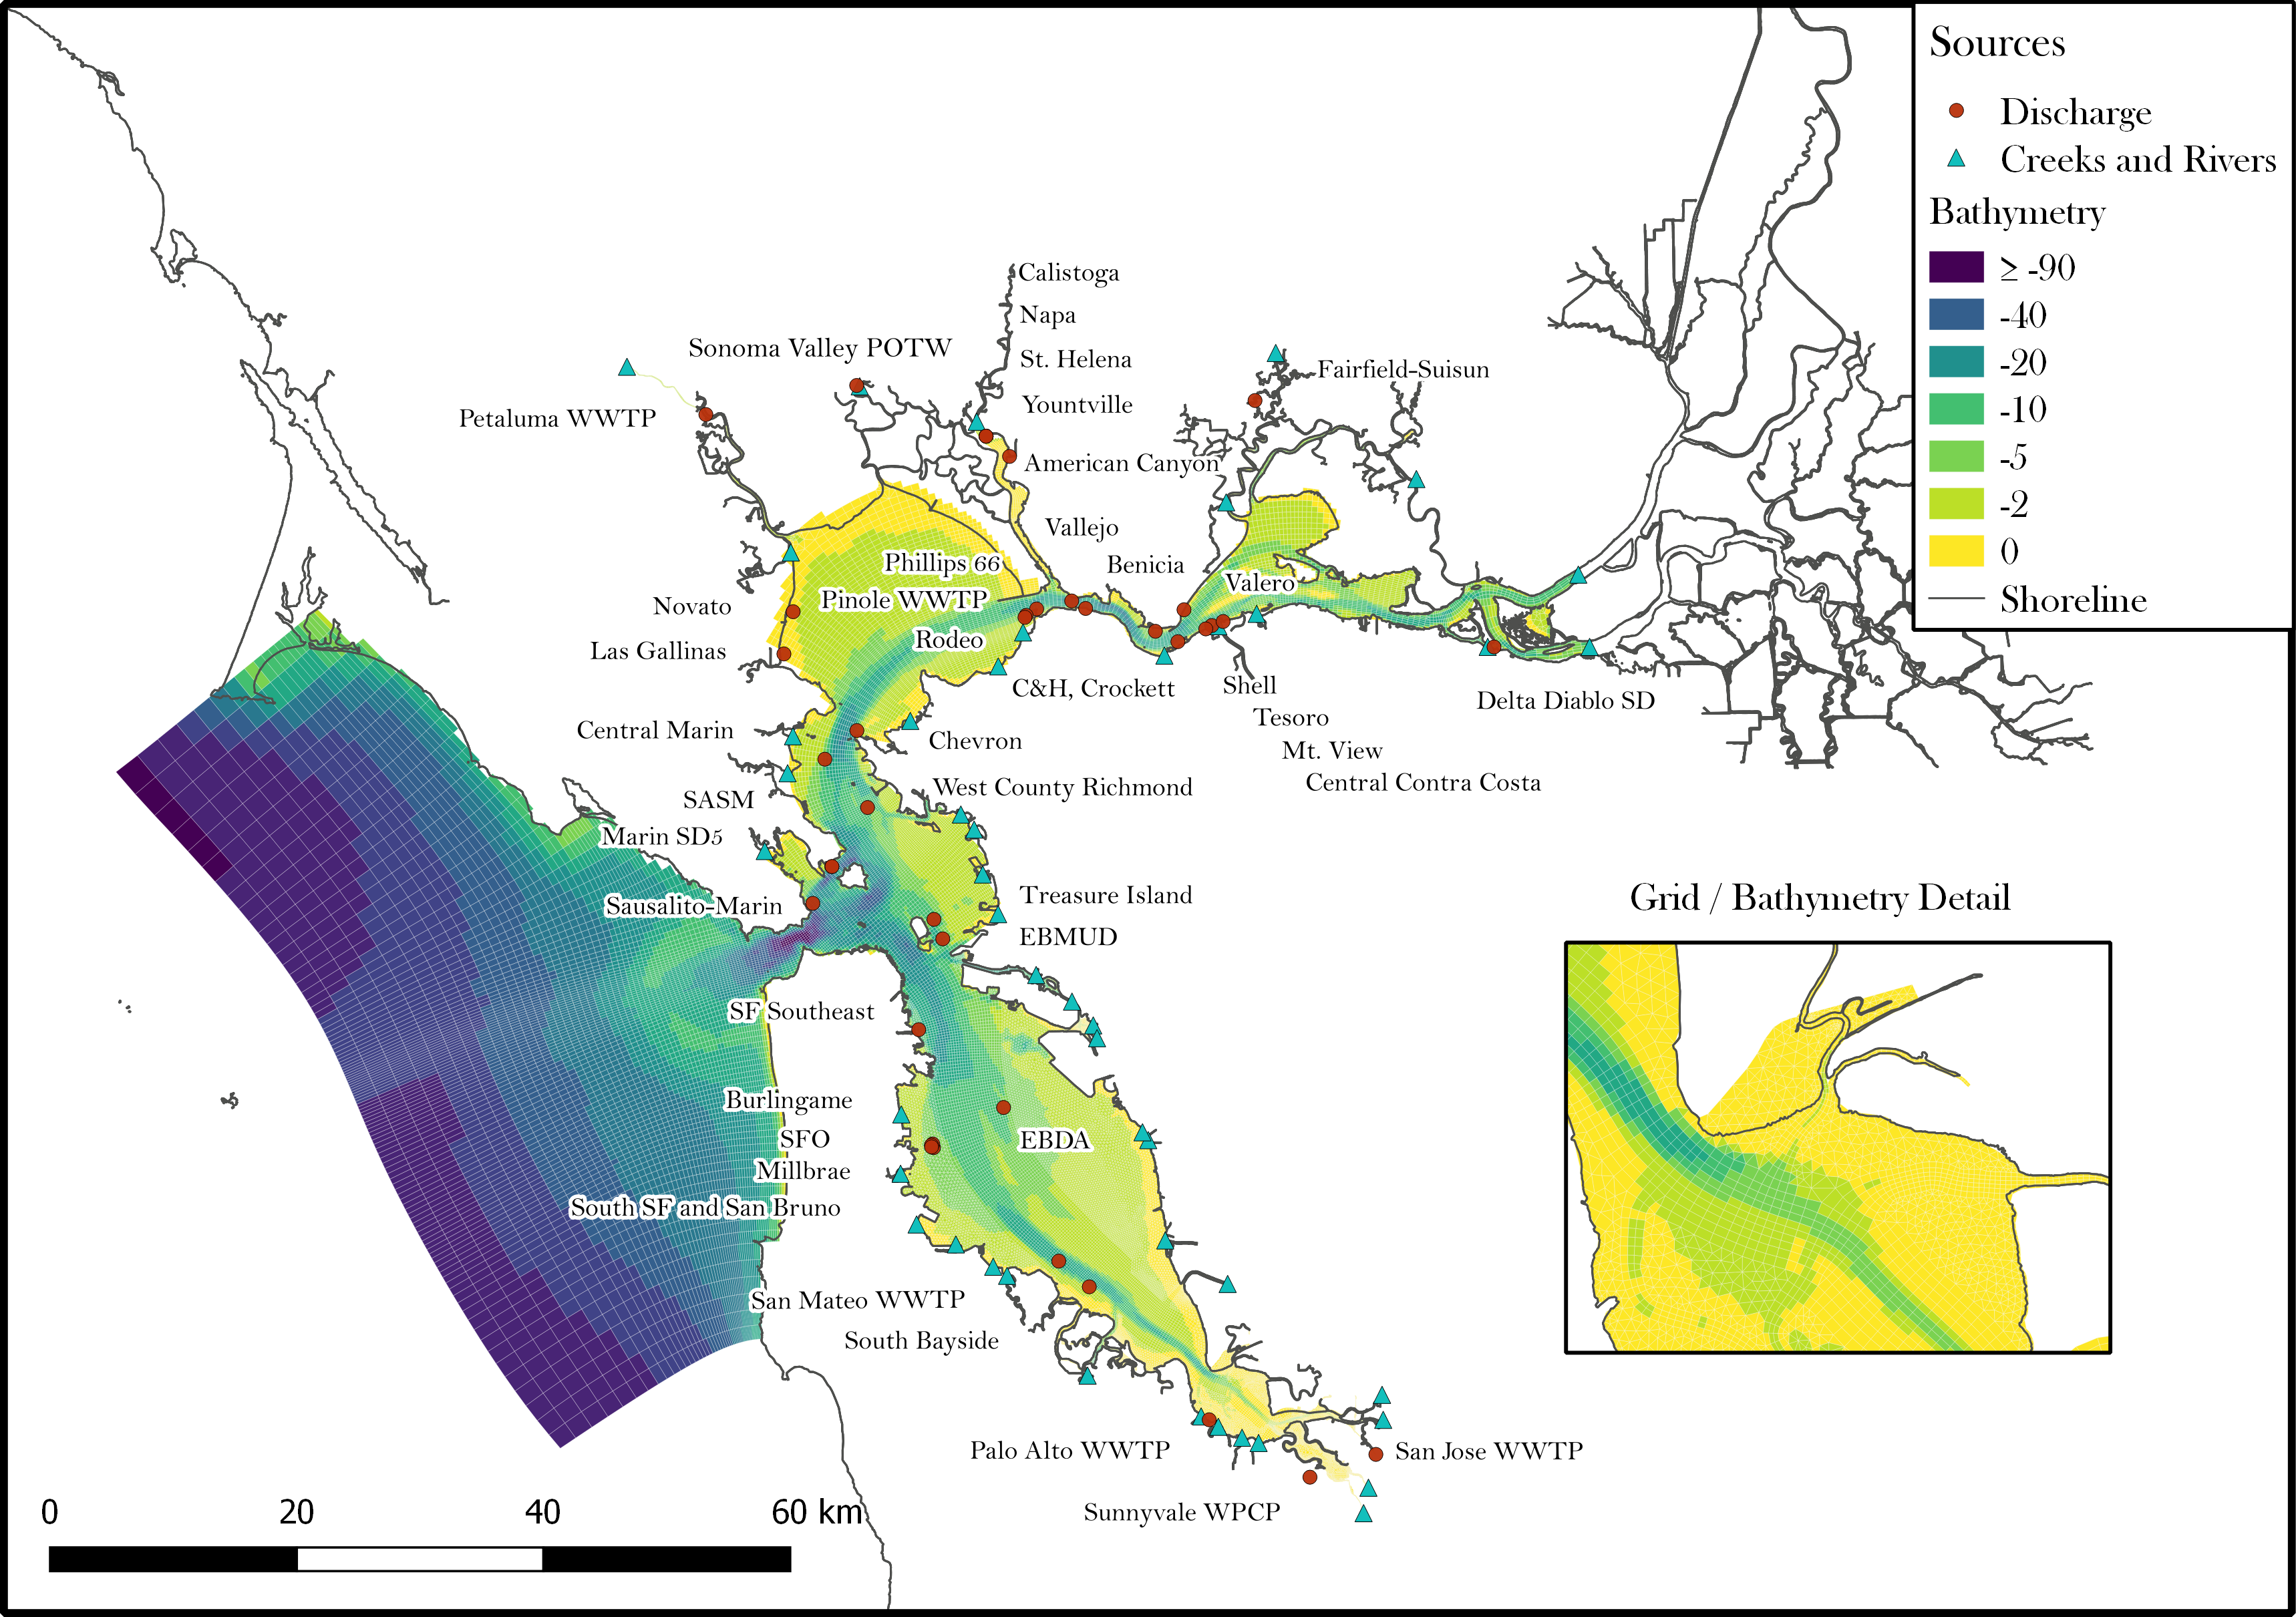
\includegraphics[width=\textwidth]{Figures/grid_inputs_v21.png}
\caption{San Francisco Bay DFM grid}
\label{fig:grid}
\end{figure}
\FloatBarrier

\subsubsection{Boundary Conditions}
The open ocean boundary is tidally forced with observed 6-minute water level data (NOAA gage 9415020), which is low-pass filtered with a 4th order Butterworth filter with a 3-hour cutoff period. Salinity at this boundary is set to a constant 33 ppt. The shorter northern and southern edges of the ocean boundary are closed.

Freshwater flows were derived from the Bay Area Hydrologic Model (a HSPF-based hydrologic model), calibrated against gage data over the 2000–2016 period. This model includes ***check this number*** 44 separate river and stormwater inputs to SFB (Fig. \ref{fig:grid}). All river and stormwater inputs are assumed to enter the Bay with negligible salinity and constant temperature of 20\(\degree\)C.

To avoid undue computational complexity the hydrodynamic model does not extend into the Sacramento-San Joaquin Delta. The edge of the model domain is at Rio Vista on the Sacramento River and Jersey Point on the San Joaquin River, well within the tidal portion of the system. Boundary conditions here are taken from USGS streamflow gages (11455420 and 11337190) for the Sacramento and San Joaquin flows, respectively. Flows at Rio Vista and Jersey Point are assumed to have negligible salinity. Water temperature is obtained from the same USGS gaging stations and assigned to in-flowing water in the model.

In parts of the Bay, especially South Bay, wastewater treatment plants (WWTPs) inputs are significant freshwater sources and influence the density field. Flow and load data for 37 WWTPs and 5 refineries have been compiled and made available online via ERDDAP (***) and github (***). This compilation draws on observed flow rates where data exist. For dates when flow data is unavailable, a flow rate is estimated based on inter-annual trends and a seasonal flow climatology. Each of the 42 inflows have been added to the hydrodynamic model as a freshwater source located at the bed.

The wind field is interpolated from 52 wind stations around SFB and specified hourly on a 1.5 km by 1.5 km grid. Specifics of the interpolation method and data sources can be found in King (2019) **cite**. 

In addition to stormwater runoff which enters the model at prescribed locations along the boundary, we also include direct precipitation and evaporation acting directly on the water surface. The model incorporates measured precipitation and evapotranspiration (ET\degree) from the CIMIS Union City station. ** rewrite, maybe don't include **

The model has been run on a Linux workstation utilizing 16 Intel Xeon E5-2680 2.40~GHz cores, communicating over MPI. DFM was compiled from SVN revision 52184 of the source code and GCC 5.4.0. 

\section{Results}\label{S:results}

\subsection{Probabilistic Analysis}
Our probabilistic analysis relies heavily on the calculated stratification metric, the horizontal Richardson number. After calculating this metric, we compared it to the cruise-averaged stratification profiles from USGS stations 24, 25, 27, and 29. Multiple stations were averaged together to minimize noise from any one station's variability and compare how the horizontal Richardson number does in capturing the aggregate stratification condition in this region of the bay. USGS cruises sample at various phases in the tide and thus observed stratification may at times be biased by ebb tide stratification due to tidal straining; however, our stratification metric tends to agree well with observed stratification (Fig. \ref{fig:rix}). Times of observed strong stratification correspond well with higher horizontal Richardson number.  

\begin{figure}[ht!]
\centering
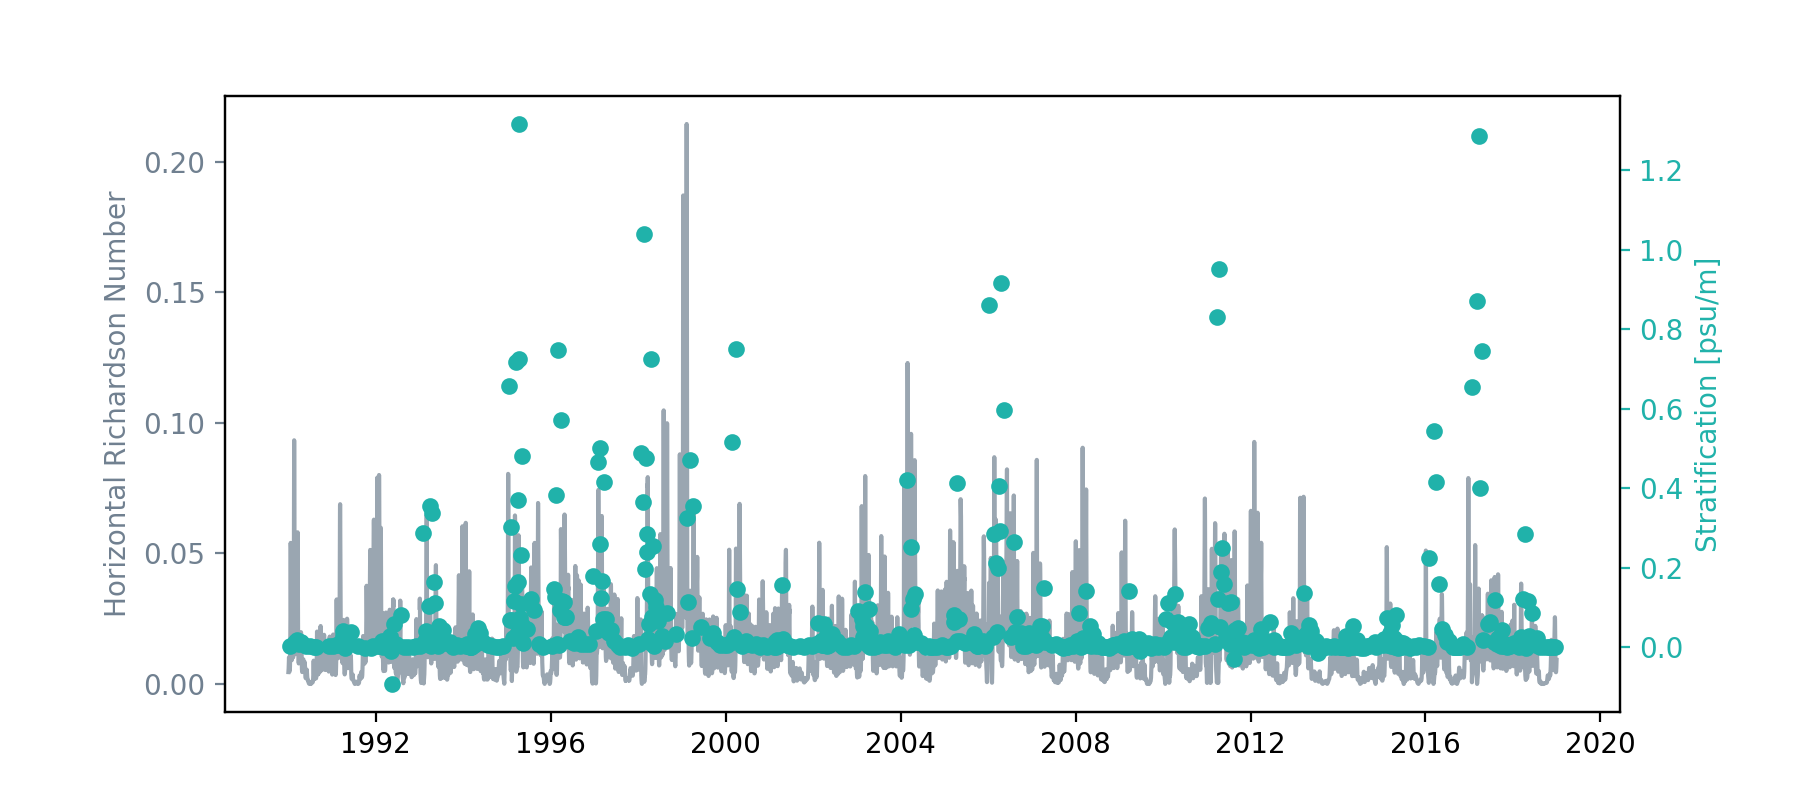
\includegraphics[width=\textwidth]{Figures/Rix_dsdz_timeseries.png}
\caption{Calculated daily horizontal Richardson number and observed average stratification between USGS stations 24, 25, 27, and 29}
\label{fig:rix}
\end{figure}
\FloatBarrier

The horizontal Richardson number was split into 9 quantiles evenly spaced between 0.05 and 0.85. Chlorophyll observations were subset by the corresponding 3-day windowed horizontal Richardson number. The n-value for each chlorophyll subset hovered around 55 for each horizontal Richardson quantile bin. The probability of observing a particular chlorophyll threshold or higher was calculated for each chlorophyll subset using varying quantile thresholds from 0.1 to 0.9. Figure \ref{fig:chl_pdf} visually shows the results of these calculations. The probability of observing a chlorophyll level in the 0.1 quantile or higher is around 0.9-1.0 for all quantiles of horizontal Richardson number. As the chlorophyll threshold is increased in the probability calculation, probabilities drop rapidly resulting in their minimum values at the highest chlorophyll threshold (quantile 0.9) ranging from approximately 0 to 0.18 as you increase in horizontal Richardson number quantile. Probabilities generally increase as you increase horizontal Richardson number and decrease as you increase chlorophyll quantile. 

\begin{figure}[ht!]
\centering
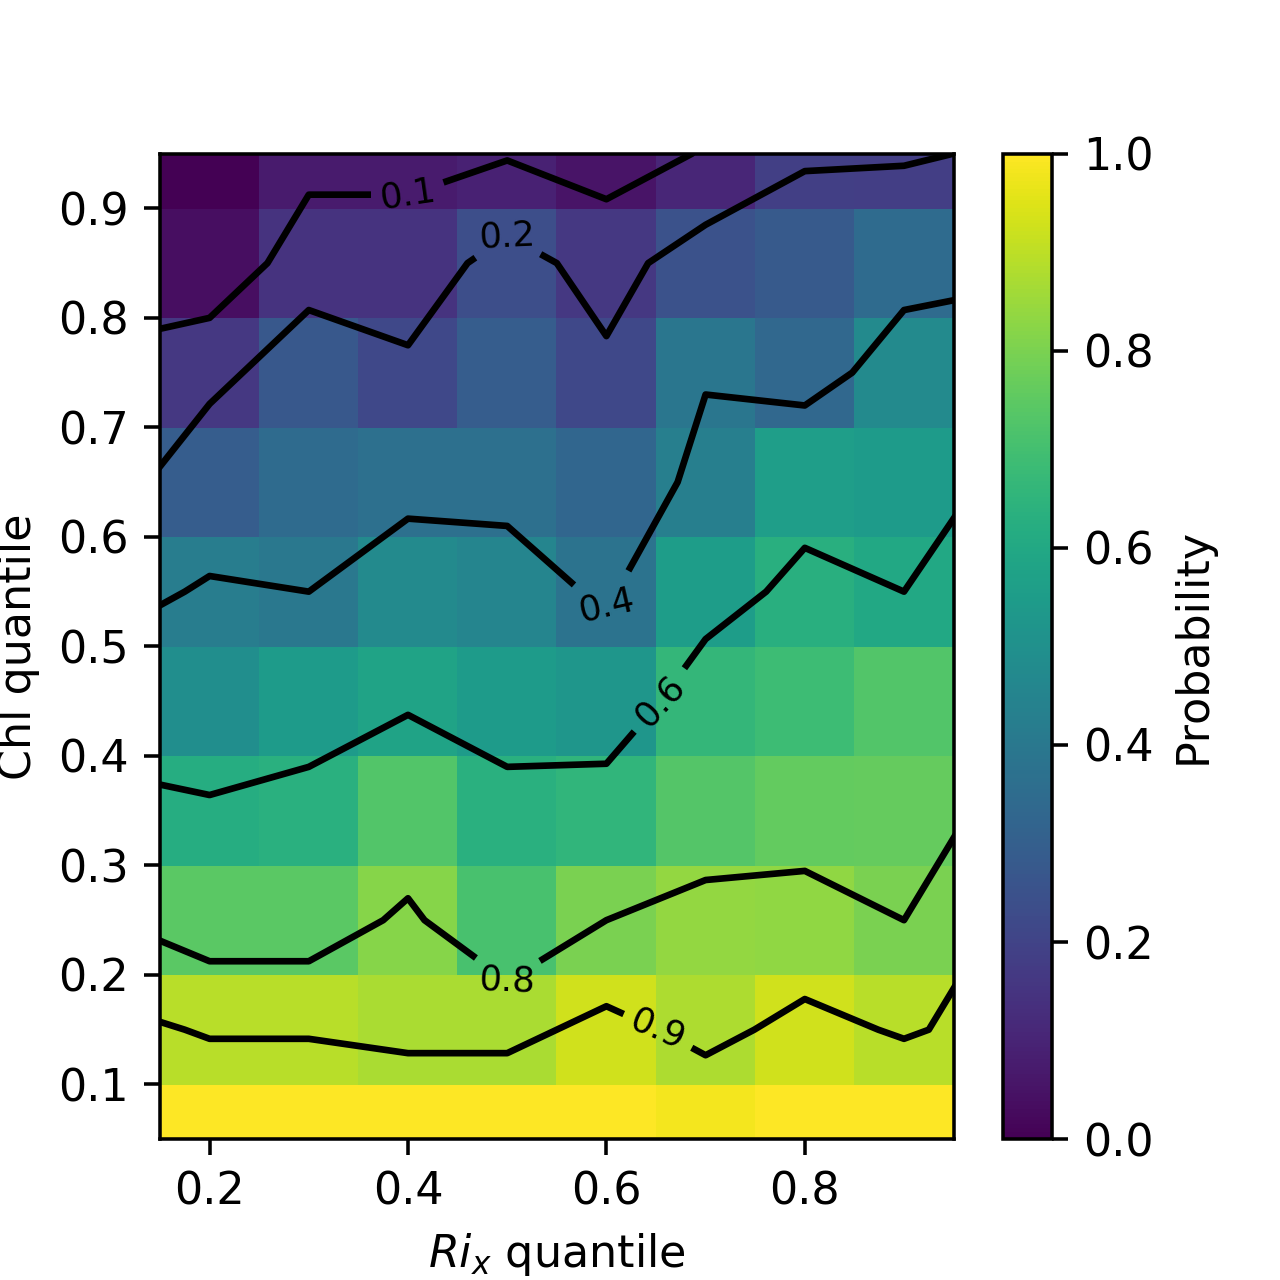
\includegraphics[width=\textwidth]{Figures/chl_rix_pdf.png}
\caption{}
\label{fig:chl_pdf}
\end{figure}
\FloatBarrier

The probability calculations made in Figure \ref{fig:chl_pdf} can be made into a continuous probability function with chlorophyll and horizontal Richardson number quantiles as inputs and a probability as output using radial basis functions. Calculated 

\subsection{Hydrodynamic Simulation}
The hydrodynamic model was run from August 2012 through September 2013 (Water Year 2013) and from August 2016 through September 2017 (Water Year 2017). For both runs, August through September were used as a two month spin up period. Validation of water level, velocity, temperature, and salinity for available locations and times provides good agreement. A detailed validation of the model setup is found in ****(sfei validation report). 



\section{Discussion}\label{S:discussion}

\section{Conclusions}\label{S:conclusion}


%% The Appendices part is started with the command \appendix;
%% appendix sections are then done as normal sections
%% \appendix

%% \section{}
%% \label{}

%% References
%%
%% Following citation commands can be used in the body text:
%% Usage of \cite is as follows:
%%   \cite{key}          ==>>  [#]
%%   \cite[chap. 2]{key} ==>>  [#, chap. 2]
%%   \citet{key}         ==>>  Author [#]

%% References with bibTeX database:

\bibliographystyle{model1-num-names}
\bibliography{bibliography.bib}

%% Authors are advised to submit their bibtex database files. They are
%% requested to list a bibtex style file in the manuscript if they do
%% not want to use model1-num-names.bst.

%% References without bibTeX database:

% \begin{thebibliography}{00}

%% \bibitem must have the following form:
%%   \bibitem{key}...
%%

% \bibitem{}

% \end{thebibliography}


\end{document}

%%
%% End of file `elsarticle-template-1-num.tex'.